\newpage
\section{TLS layers}

\tlsI{} is a layered protocol, and consists of the Record Protocol,
the Handshake Protocol and the Alert Protocol. The Record Protocol
is to serve all other protocols and is above the transport layer.
The Record protocol offers symmetric encryption, and data authenticity.
In \gnutls{} the record protocol is accessed using the 
\hyperref{gnutls\_record\_read()}{gnutls\_record\_read() (see Section }{)}{gnutls_record_read} and
\hyperref{gnutls\_record\_write()}{gnutls\_record\_write() (see Section }{)}{gnutls_record_write}
functions.

\par
The Alert protocol offers some signaling to the other protocols. It can
help informing the peer for the cause of failures and other error
conditions.
\hyperref{gnutls\_alert\_send()}{gnutls\_alert\_send() (see Section }{)}{gnutls_alert_send} and
\hyperref{gnutls\_alert\_send\_appropriate()}{gnutls\_alert\_send\_appropriate() (see Section }{)}{gnutls_alert_send_appropriate} 
functions.

\par 
The Handshake protocol is responsible for the initial key exchange,
and authentication. See \hyperref{figure}{figure }{}{fig:cert} for the
protocol layering in TLS. The handshake protocol in \gnutls{} is accessed
with the 
\hyperref{gnutls\_handshake()}{gnutls\_handshake() (see Section }{)}{gnutls_handshake} function.

\begin{figure}[hbtp]
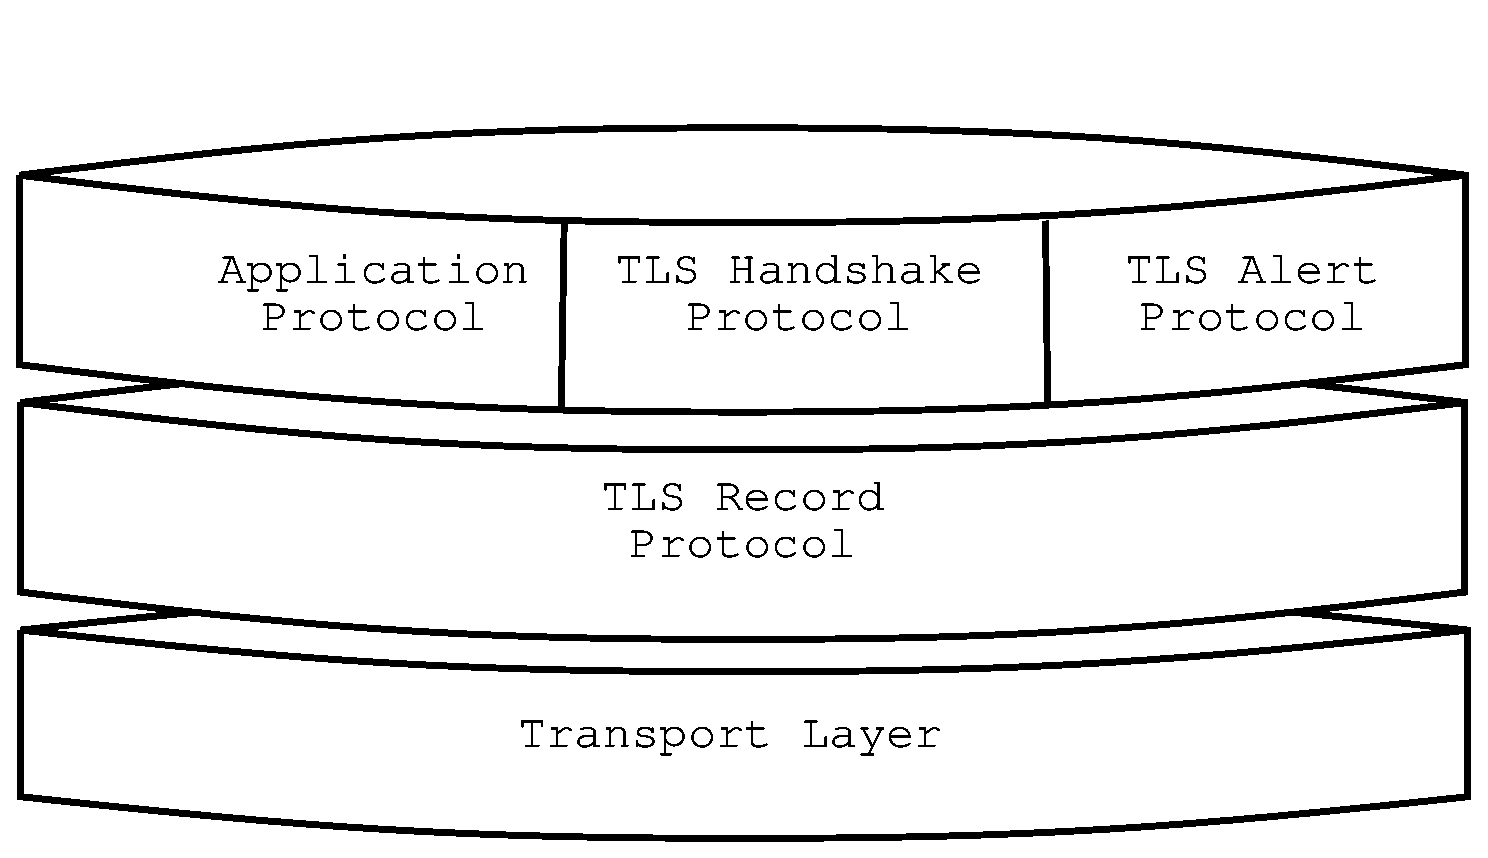
\includegraphics{layers}
\label{fig:layers}

\end{figure}


\addvspace{1.5cm}

